\documentclass[article]{jss}
\usepackage[utf8]{inputenc}

\providecommand{\tightlist}{%
  \setlength{\itemsep}{0pt}\setlength{\parskip}{0pt}}

\author{
Ítalo Ramos Cegatta\\University of São Paulo \And Cristian Villegas\\University of São Paulo
}
\title{comp3: um pacote em \proglang{R} para índices de competição em árvores
indivuais}
\Keywords{floresta, índice de competição, árvore individual, \proglang{R}}

\Abstract{
The abstract of the article.
}

\Plainauthor{Ítalo Ramos Cegatta, Cristian Villegas}
\Plaintitle{comp3}
\Shorttitle{comp3: um pacote em \proglang{R} para índices de competição em árvores
indivuais}
\Plainkeywords{floresta, índice de competição, árvore individual, R}

%% publication information
%% \Volume{50}
%% \Issue{9}
%% \Month{June}
%% \Year{2012}
\Submitdate{}
%% \Acceptdate{2012-06-04}

\Address{
    Ítalo Ramos Cegatta\\
  University of São Paulo\\
  First line Second line\\
  E-mail: \href{mailto:italocegatta@gmail.com}{\nolinkurl{italocegatta@gmail.com}}\\
  URL: \url{http://italocegatta.github.io}\\~\\
    }

\usepackage{amsmath}

\begin{document}

\section{Introdução}\label{introducao}

A construção de modelos de crescimento é essencial para o planejamento
florestal. Independente da abordagem do modelo, seja ele baseado em
processo, empírico ou híbrido, o objetivo é representar o crescimento de
árvores e povoamentos através de formulações matemáticas (BURKHART;
TOMÉ, 2012).

O crescimento de árvores individuais é influenciado por fatores como
idade, tamanho, microambiente, características genéticas e competição
(TOMÉ, 1988). Os modelos que representam este crescimento podem ser
construídos em função da idade, índice de sítio e o status competitivo,
sendo este último o mais difícil de ser definido e mensurado
quantitativamente (ZHANG; BURKHART; AMATEIS, 1996).

A competição pode ser definida pela interação entre indivíduos que
competem por recursos e por esse motivo há redução de sobrevivência,
crescimento e reprodução (BEGON; TOWNSEND; HARPER, 2006).

Entende-se que existem 3 motivos pelos quais se justificam o estudo da
competição no componente arbóreo de uma floresta: (i) como suporte às
decisões de manejo, onde informações facilmente coletadas em campo
indicam o potencial de crescimento após uma interferência silvicultural;
(ii) para entender qual a ordem e grandeza de influência de fatores como
água, luz, densidade populacional e nutrientes no crescimento de uma
árvore no povoamento; (iii) para a utilização de índices de competição
em modelos de predição com estimativa acurada do incremento em diâmetro
e altura das árvores (MORAVIE; DURAND; HOULLIER, 1999).

Em um modelo de crescimento de árvore individual, o índice de competição
caracteriza o grau em que o espaço disponível para crescimento de uma
planta é compartilhado pelas suas vizinhas (BURTON, 1993; RADTKE;
WESTFALL; BURKHART, 2003). A avaliação da performance dos índices de
competição é comumente realizada através da correlação do índice com o
incremento em diâmetro, área basal e altura (DANIELS; BURKHART; CLASON,
1986). Diversos autores, ao modelar o crescimento e a produção,
obtiveram ganhos na qualidade do ajuste ao incluir índices de competição
no modelo (MORAVIE; DURAND; HOULLIER, 1999; SCHRÖDER; GADOW, 1999;
SOARES; TOMÉ, 1999; CONTRERAS; AFFLECK; CHUNG, 2011; FRAVER et al.,
2014)

É comum na literatura a classificação dos índices de competição em dois
grupos: dependentes e independentes da distância (MALEKI; KIVISTE;
KORJUS, 2015). Índices independentes da distância não necessitam das
coordenadas das árvores, uma vez que são simples cálculos envolvendo
variáveis do povoamento e da árvore-objeto. Já os dependentes da
distância consideram as dimensões e localização parcial dos vizinhos
competidores para o cálculo do índice. Para este índice, também é
necessário um critério que define quais árvores são competidoras em
relação a uma data árvore-objeto. (SOARES; TOMÉ, 1999; RIVAS et al.,
2005).

\section{The comp3 package}\label{the-comp3-package}

O software R é um ambiente computacional para desenvolvimento de
análises estatísticas e gráficas (R CORE TEAM, 2016), a linguagem dispõe
de várias funções para análises de dados e ainda possibilita utilizar
funções disponíveis em pacotes criados por outros usuários. O CRAN,
principal repositório de pacotes da linguagem R possui poucos pacotes
direcionados para resolução de problemas da área florestal, com destaque
para os pacotes \emph{FAwR} e \emph{lmfor}. O pacote \emph{comp3} foi
desenvolvido com o objetivo de disponibilizar funções que facilitam o
cálculo de índices de competição de árvores individuais de um povoamento
florestal. Estão implementados os principais índices de competição tanto
para florestas plantadas quanto para florestas naturais. A concepção das
funções do pacote sugere um fluxo de trabalho para o calculo dos
índices, que envolve:

\begin{itemize}
\item
  criação de coordenadas locais para árvores que estejam dispostas em
  parcelas rigorosamente esquadrejada;
\item
  delimitação da faixa de bordadura da parcela, que identifica as
  árvores como úteis para análise e as árvores de bordadura;
\item
  determinação das árvores competidoras para cada árvore-objeto;
\item
  cálculo de índices dependentes ou independentes da distância.
\end{itemize}

\subsection{Coordenadas locais}\label{coordenadas-locais}

Caso o banco de dados não possua a disposição espacial das árvore, mas
se sabe que as árvores da parcela amostral foram plantadas com extremo
rigor e esquadrejamento, é possível criar um grid hipotético e assim
gerar coordenadas locais para as árvores da parcela.

O exemplo abaixo exemplifica a criação de coordenadas para um conjunto
de dados hipotéticos. Pretende-se criar as coordenadas x e y de 25
árvores que pertencem a uma parcela de 5 linhas por 5 plantas. A
identificação de cada árvore é data pelo caminhamento em zig-zag pela
parcela. As funções \emph{xcoord} e \emph{ycoord} criam as coordenadas
locais a partir do identificador da árvore, podendo ele ser numérico ou
textual. É preciso especificar o arranjo de plantio e o número de linhas
que a parcela possui. Por fim, é definido o início do caminhamento,
podendo ser escolhido um dos quatro vértices da parcela.

\begin{CodeChunk}
\begin{CodeInput}
library(tidyverse)
library(comp3)

foo <- data_frame(id = 1:25) %>% 
  mutate(
    x = xcoord(x = id, xspacing =  2, ncol =  5, star = "left-bottom"),
    y = ycoord(x = id, yspacing =  2, ncol =  5, star = "left-bottom")
  ) 

foo %>% 
  ggplot(aes(x, y, label = id)) +
  geom_label(size = 4)
\end{CodeInput}


\begin{center}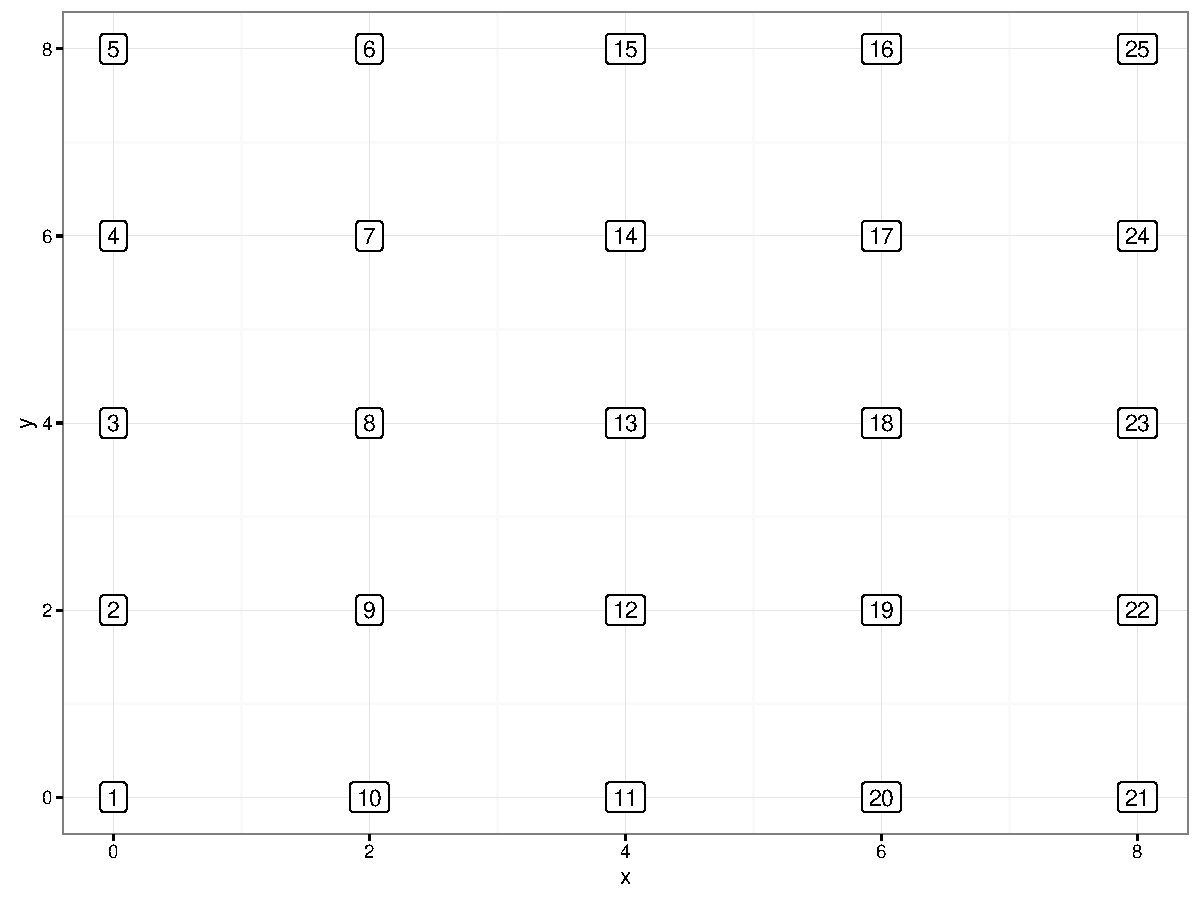
\includegraphics{comp3-paper_files/figure-latex/unnamed-chunk-2-1} \end{center}

\end{CodeChunk}

Caso todas as árvores da parcela possuírem coordenadas, é possivel
delimitar uma faixa de bordadura para garantir que as árvores estudadas
estejam livres de influência externa.

A função \emph{avaliable\_tree} retorna, a partir das coordenadas e do
tamanho da bordadura, um vetor lógico que identifica as árvores úteis
(TRUE) e de borda (FALSE).

\begin{CodeChunk}
\begin{CodeInput}
foo %>% 
  mutate(borda = available_tree(x = x, y = y, border = 2)) %>% 
  ggplot(aes(x, y, label = id, color = borda)) +
  geom_point(size = 4) +
  labs(color = "`Árvore útil") +
  scale_colour_manual(
    values = c("FALSE" = "#d95f02", "Objeto" = "#7570b3", "TRUE" = "#1b9e77")
  ) +
  theme(legend.position = "top")
\end{CodeInput}


\begin{center}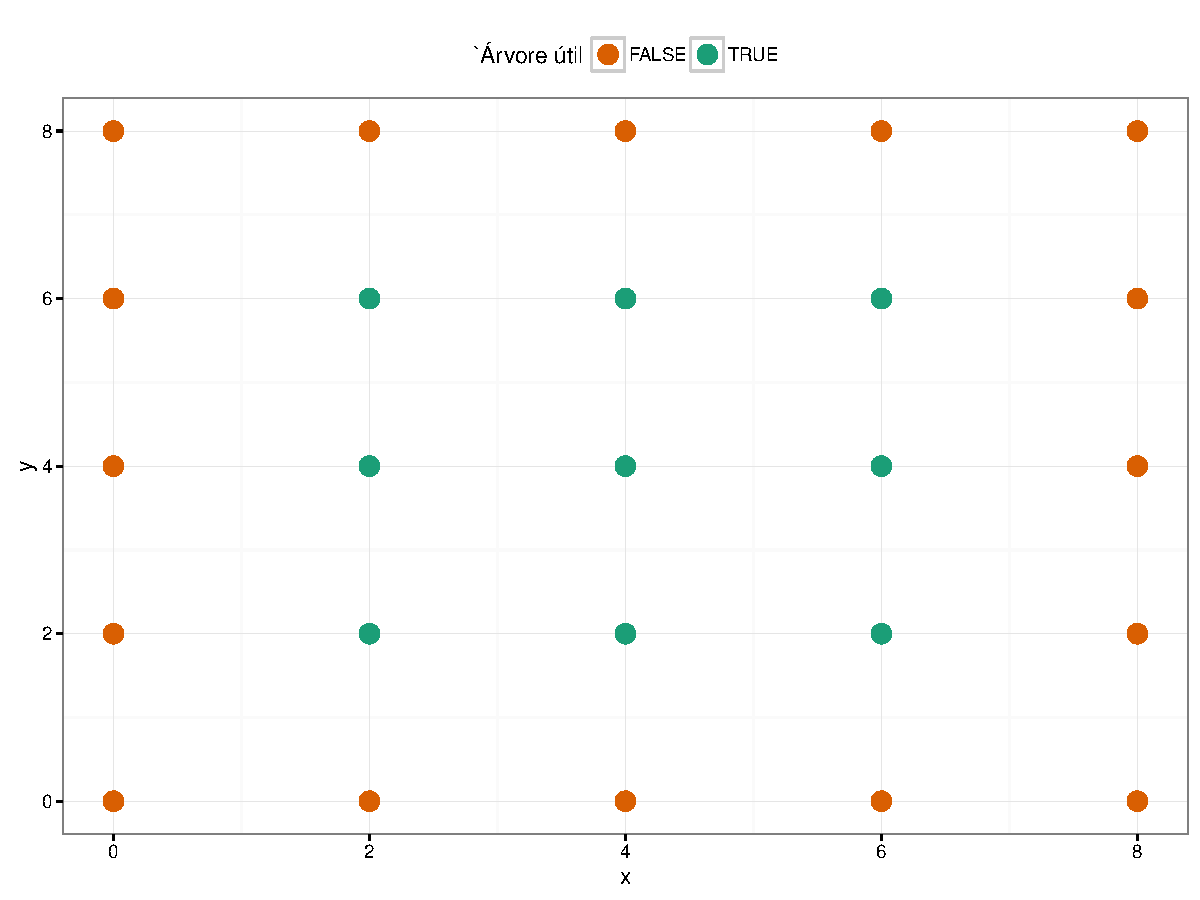
\includegraphics{comp3-paper_files/figure-latex/unnamed-chunk-3-1} \end{center}

\end{CodeChunk}

\subsection{Árvores competidoras}\label{arvores-competidoras}

A determinação de uma árvore competidora ocorre somente nos índices de
competição dependentes da distancia, uma vez que nos indices
independentes da distância entende-se que todas as árvores da parcela
contribui igualmente para o status competitivo do povoamento. O pacote
fornece duas opções para a escolha do competidor, o primeiro delimita um
raio de busca e seleciona todas as árvores que estão dentro desta faixa.
A Figura 1 mostra 25 árvores hipotéticas, dispostas de maneira regular.
A partir da árvore objeto, todas as árvores vizinhas que estiverem
dentro do circulo com raio de 2,5 m são consideradas como competidoras.
A determinação do raio de busca ou do número de arvores mais próximas é
determinada pelo pesquisador e tem impacto relevante no cálculo dos
índices dependentes da distância. O segundo estabelece um rank de
distância entre as árvores-objeto e suas possíveis competidoras e
seleciona o número de árvores de acordo com o parâmetro especificado na
função.

\begin{CodeChunk}


\begin{center}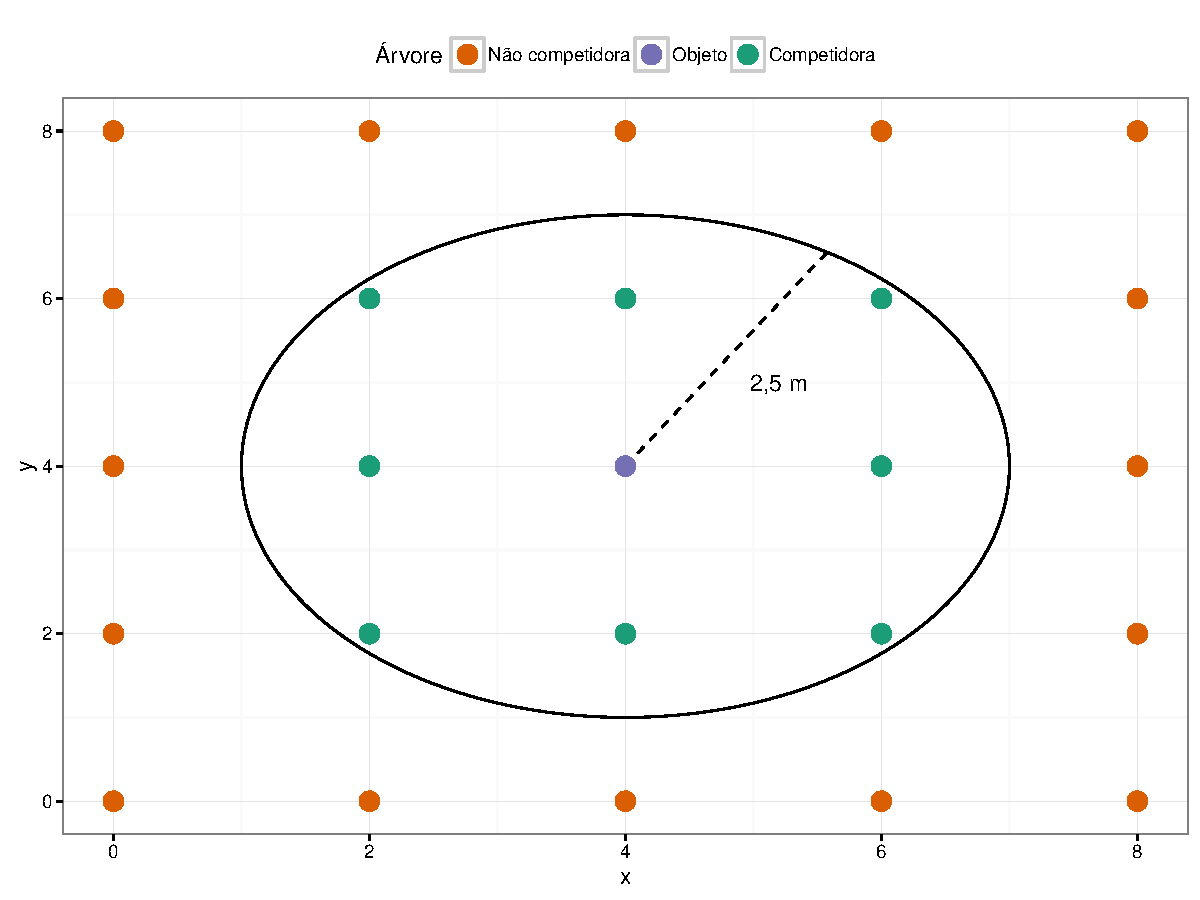
\includegraphics{comp3-paper_files/figure-latex/unnamed-chunk-4-1} \end{center}

\end{CodeChunk}

As funções dos índices dependentes da distância calculam através da
função \emph{search\_nearest} , internamente os competidores para cada
árvore-objeto, de modo que a expressão de cálculo dos índices são
aplicadas apenas a estas árvores. A função retorna, para cada
árvore-objeto, seus competidores e a distâcnia entre os dois.

\subsection{Índices de competição}\label{indices-de-competicao}

Foram implementados índices dependentes e independentes da distância.
Cada índice, identificado com o nome do autor que o propôs, tem uma
função própria e é calculado individualmente. Os índices independentes
da distância necessitam obrigatoriamente do diâmetro das árvores e
eventualmente da área da parcela amostral. Já os índices dependentes da
distância exigem além do diâmetro, as coordenadas das árvores em um
plano cartesiano, seja ele real ou hipotético, e do método que considera
uma árvore vizinha como competidora.

\section{Estudo de caso}\label{estudo-de-caso}

O pacote \emph{comp3} diponibiliza um banco de dados com medições
sucessivas de um plantio experimental de \emph{Eucalyptus}. Trata-se de
um plantio clonal, implantado em 4 locais diferentes com extremo rigor
silvicultural. A parcela de medição possui 8 linhas por 10 plantas, com
arranjo de plantio de 3 x 3 m e, onde foram mensuradas em todas as
árvores o diâmetro a 1,3 m, altura total, altura do início da copa e
atributos qualitativos. A drescição completa pode ser vista na descrição
do banco de dados em \texttt{?eucalyptus}. A Figura XX mostra o as
médias das variáveis avaliadas em cada medição nos 4 sítios estudados.

\begin{CodeChunk}

\begin{tabular}{r|r|r|r|r|r}
\hline
site & area & age & dbh & h & cbh\\
\hline
4 & 720 & 15 & 8.6 & 11.4 & 0.8\\
\hline
4 & 720 & 21 & 9.9 & 13.5 & 8.9\\
\hline
4 & 720 & 27 & 12.4 & 15.0 & 9.6\\
\hline
4 & 720 & 33 & 13.0 & 17.7 & 10.1\\
\hline
4 & 720 & 39 & 13.6 & 19.5 & 11.5\\
\hline
4 & 720 & 45 & 14.1 & 20.9 & 14.5\\
\hline
4 & 720 & 51 & 14.6 & 23.7 & 18.4\\
\hline
15 & 720 & 14 & 5.9 & 6.9 & 1.5\\
\hline
15 & 720 & 20 & 7.6 & 9.8 & 2.9\\
\hline
15 & 720 & 27 & 10.3 & 13.4 & 5.2\\
\hline
15 & 720 & 31 & 11.1 & 15.9 & 10.1\\
\hline
15 & 720 & 38 & 11.9 & 16.5 & 11.9\\
\hline
15 & 720 & 43 & 12.6 & 17.2 & 14.5\\
\hline
15 & 720 & 50 & 14.0 & 19.3 & 15.0\\
\hline
20 & 720 & 14 & 8.6 & 9.5 & 0.5\\
\hline
20 & 720 & 20 & 11.1 & 13.6 & 7.0\\
\hline
20 & 720 & 26 & 12.5 & 17.3 & 10.2\\
\hline
20 & 720 & 31 & 13.1 & 18.2 & 11.2\\
\hline
20 & 720 & 37 & 14.4 & 19.1 & 12.6\\
\hline
20 & 720 & 47 & 15.2 & 22.5 & 16.9\\
\hline
20 & 720 & 50 & 15.7 & 24.0 & 18.2\\
\hline
24 & 720 & 15 & 8.4 & 8.5 & 0.5\\
\hline
24 & 720 & 21 & 10.9 & 12.5 & 5.1\\
\hline
24 & 720 & 27 & 12.6 & 15.4 & 7.9\\
\hline
24 & 720 & 33 & 13.3 & 16.7 & 10.4\\
\hline
24 & 720 & 40 & 14.7 & 19.4 & 11.5\\
\hline
24 & 720 & 45 & 15.6 & 21.7 & 14.4\\
\hline
24 & 720 & 52 & 16.6 & 24.3 & 19.9\\
\hline
\end{tabular}

\end{CodeChunk}

Iniciando uma análise exploratória dos dados, podemos ver nas figuras ZZ
o crescimento em área basal do clone nos 4 sítios. Pode-se notar que o
crescimento a taxa de crescimento é semelhante entre os sítios, porém o
patamar de produção de cada sítio se diferencia, podendo-se destacar o
sítio 24 como o mais produtivo e o sítio 15 como o menos produtivo até
os 50 meses de idade.

\begin{CodeChunk}


\begin{center}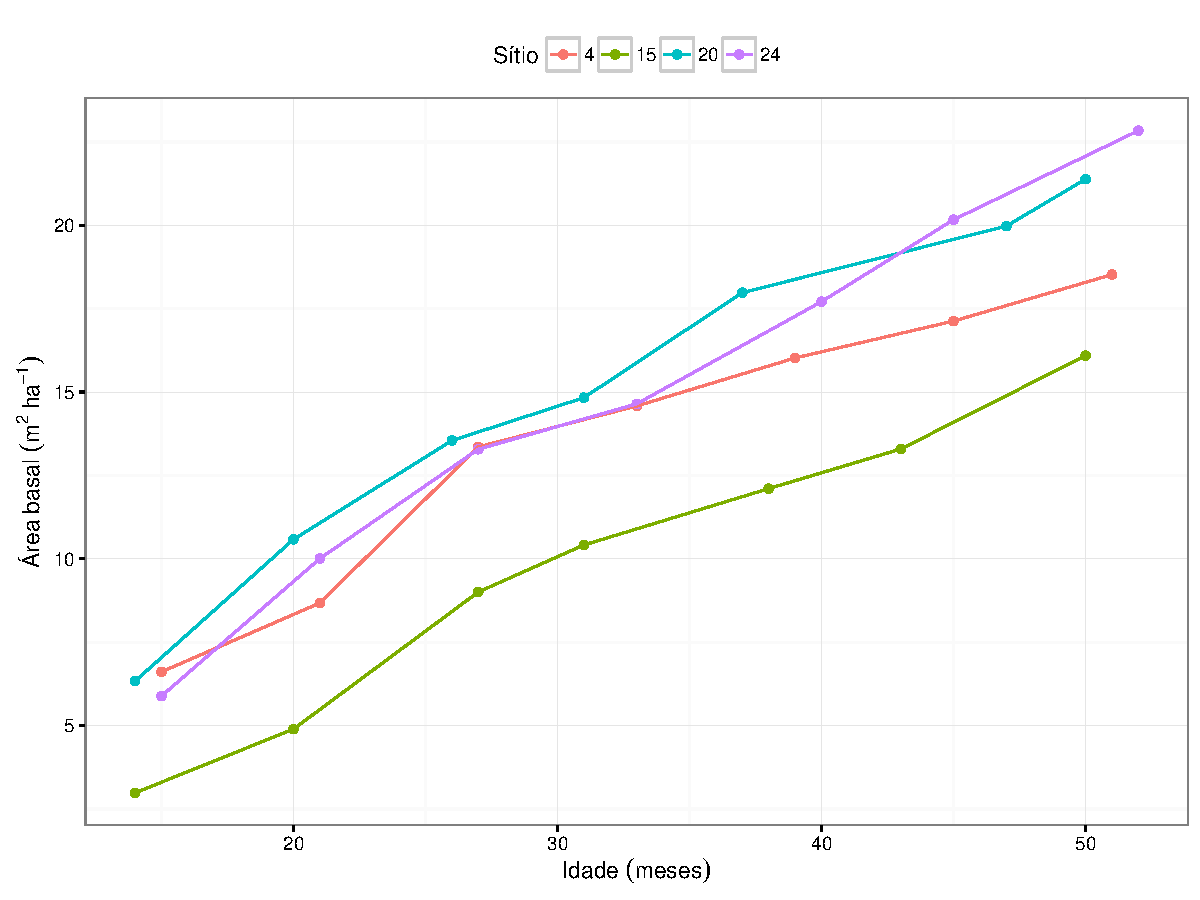
\includegraphics{comp3-paper_files/figure-latex/unnamed-chunk-8-1} \end{center}

\end{CodeChunk}

Iniciando processamento dos dados para o cálculo dos índices de
competição, será preciso criar as coordenadas locais para as árvores do
banco de dados, bem como criar uma faixa de bordadura equivalente a duas
linhas de plantio e duas plantas, conforme indica a Figura QQ.

\begin{CodeChunk}
\begin{CodeInput}
base <- eucalyptus %>% 
  group_by(site, age) %>% 
  mutate(
    x = xcoord(x = tree, xspacing =  3, ncol =  8, star = "left-bottom"),
    y = ycoord(x = tree, yspacing =  3, ncol =  8, star = "left-bottom"),
    available = available_tree(x, y, 6)
  ) 
\end{CodeInput}
\end{CodeChunk}

\begin{CodeChunk}


\begin{center}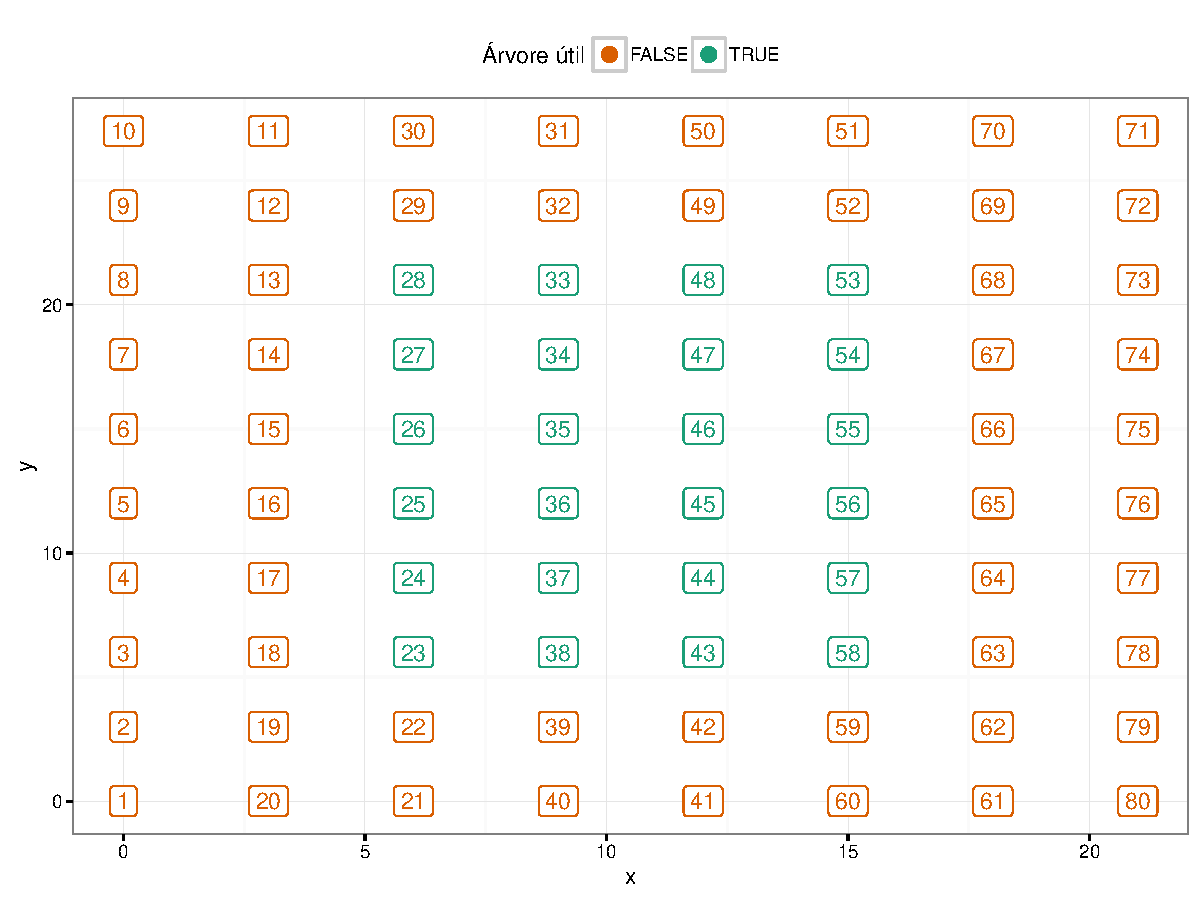
\includegraphics{comp3-paper_files/figure-latex/unnamed-chunk-10-1} \end{center}

\end{CodeChunk}

O cálculo dos índices é aseguir, onde são computados 4 índices
dependentes da distância e 6 índices independentes da distância. Para os
índices dependentes da distancia foi padronizada seleção de competidores
pelo crítério das 6 árvores mais próximas da árvore-objeto. Também foi
calculado o incremento corrente da sessão transversal de cada árvore,
com o objetivo de correlacioná-la com os índices de competição.

A Figura WW apresenta um gráfico de dispensão do valor calculado para
cada índice em função do incremento em sessão transversal.Alguns índices
foram sensíveis às árvores dominadas e tiveram resultados que podem
prejudicar a relação com o incremento da árvore. Entretando, nesta
primeira etapa, estão incluídas todas as árvores úteis do banco de
dados, podendo melhorar a visualização após a diferenciação por sítio e
idade.

\begin{CodeChunk}


\begin{center}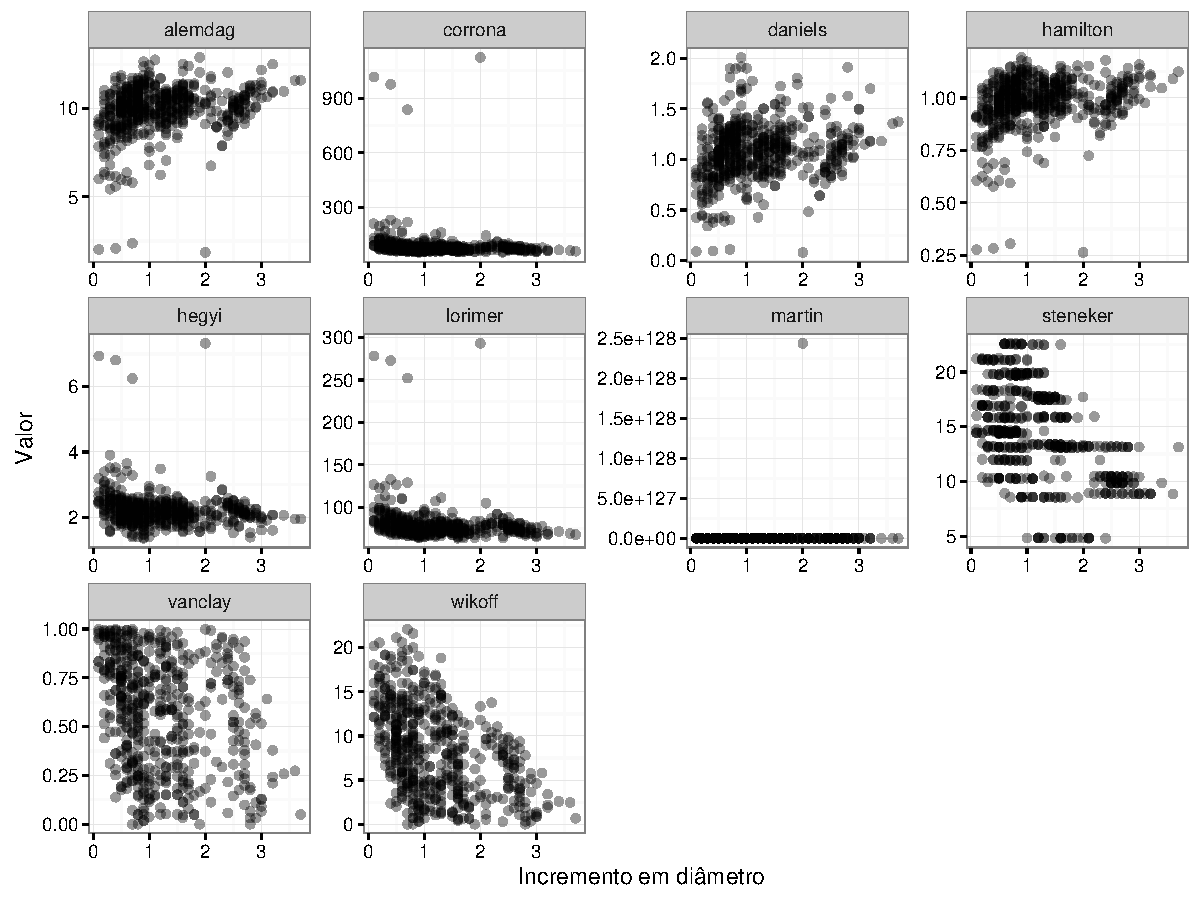
\includegraphics{comp3-paper_files/figure-latex/unnamed-chunk-12-1} \end{center}

\end{CodeChunk}

A primeira análise quantitativa será feita atravéz da correlação simples
de Pearson entre o incremento em sessão transversal e o índice de
competição. A corelação será calculada para cada sitio e idade, para
ferificar qual índice possui maior consistência de correlação em função
da idade.

O resultado das correlações estão apresentados na Figura RR. É possível
notar que em determinadas idades, todos os índices tem baixa correlação
com o incremento em diâmetro, com destaque para as medições referentes
as idade 33 e 45 meses do sítio 24, onde nenhum índice obteve correlação
maior que 0,5.

{[}buscar resultados de outros trabalhos para comparação{]}

\begin{CodeChunk}


\begin{center}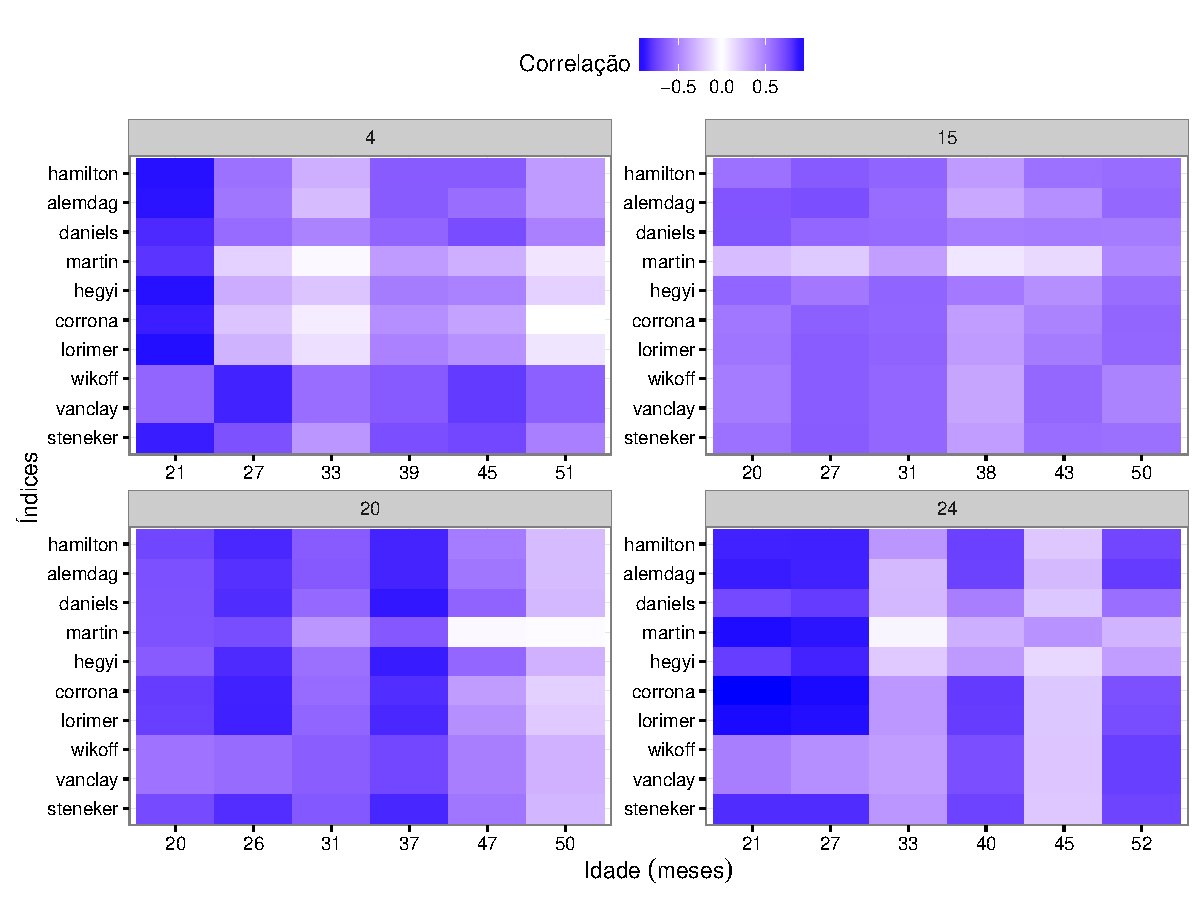
\includegraphics{comp3-paper_files/figure-latex/unnamed-chunk-14-1} \end{center}

\end{CodeChunk}

Será feito uma breve análise dos 4 índices que obtiveram melhores
resultados em termos de correlação com o incremento.

\subsection{}\label{section}

\begin{CodeChunk}
\begin{CodeInput}
base_index_sml %>% 
  filter(index == "steneker") %>% 
  ggplot(aes(cai, value, color = age %>% factor)) +
    geom_point(alpha = 0.4) +
    facet_wrap(~site) +
    labs(x = ~Incremento~em~diâmetro, y = ~Valor)
\end{CodeInput}


\begin{center}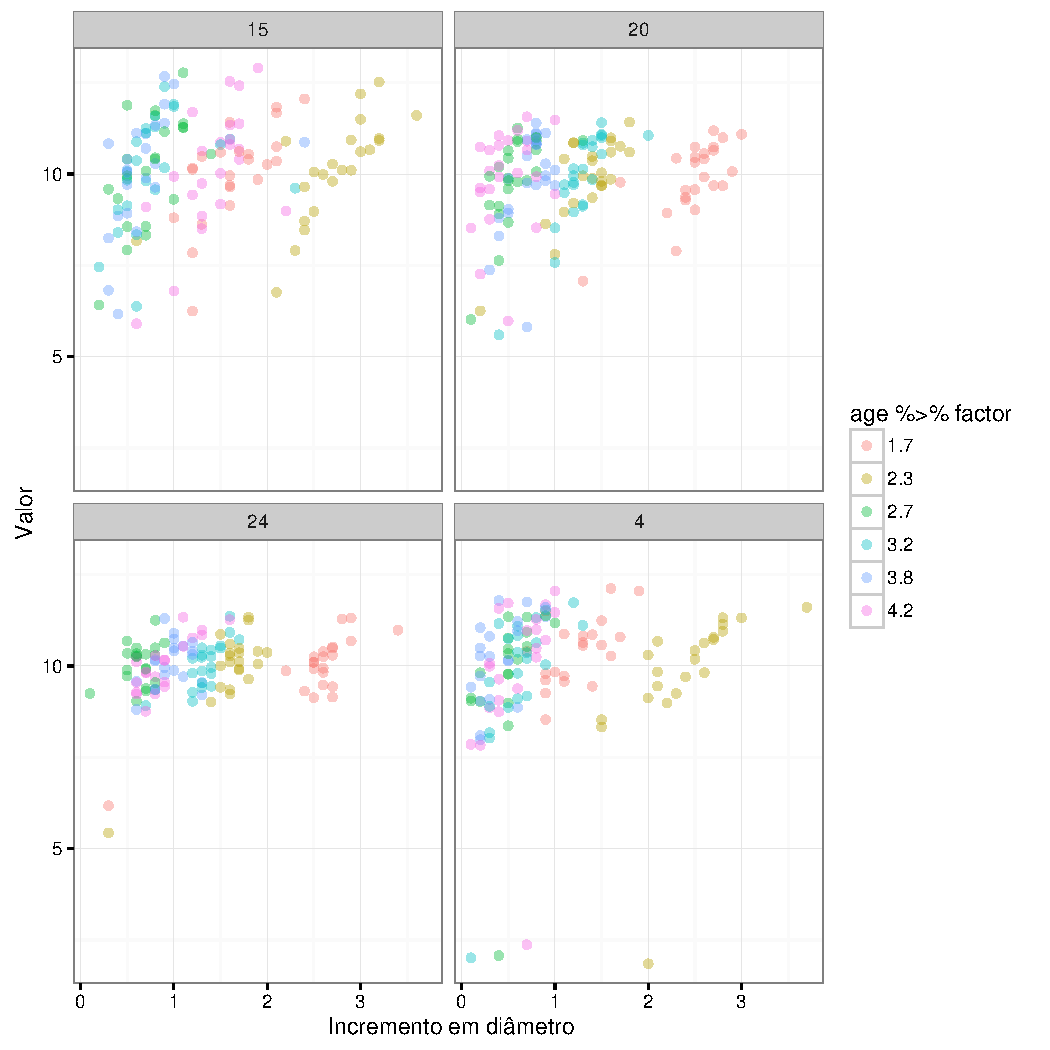
\includegraphics{comp3-paper_files/figure-latex/unnamed-chunk-16-1} \end{center}

\end{CodeChunk}

\begin{CodeChunk}
\begin{CodeInput}
base_index_sml %>% 
  filter(index == "alemdag") %>% 
  ggplot(aes(cai, value, color = age %>% factor)) +
    geom_point(alpha = 0.4) +
    facet_wrap(~site) +
    labs(x = ~Incremento~em~diâmetro, y = ~Valor)
\end{CodeInput}


\begin{center}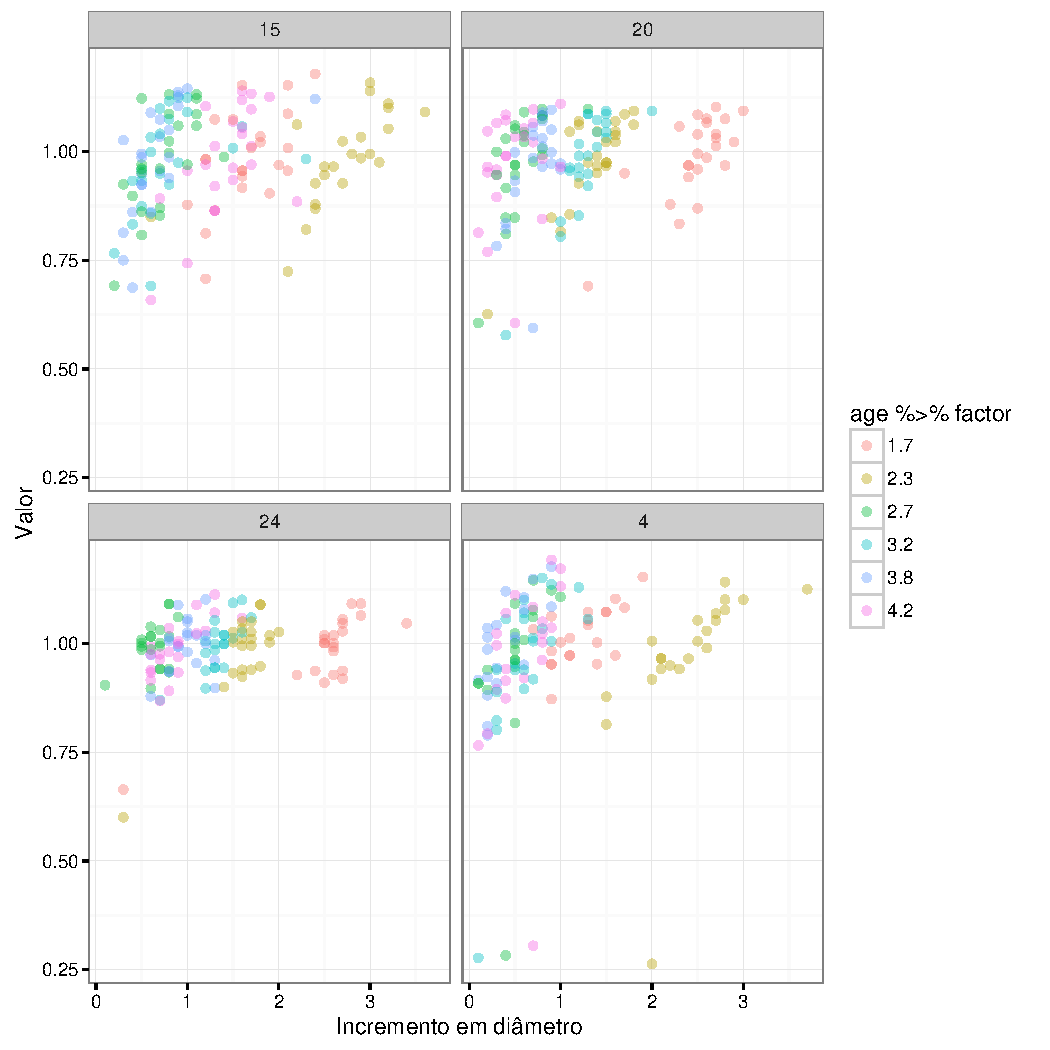
\includegraphics{comp3-paper_files/figure-latex/unnamed-chunk-17-1} \end{center}

\end{CodeChunk}

\begin{CodeChunk}
\begin{CodeInput}
base_index_sml %>% 
  filter(index == "hamilton") %>% 
  ggplot(aes(cai, value, color = age %>% factor)) +
    geom_point(alpha = 0.4) +
    facet_wrap(~site) +
    labs(x = ~Incremento~em~diâmetro, y = ~Valor)
\end{CodeInput}


\begin{center}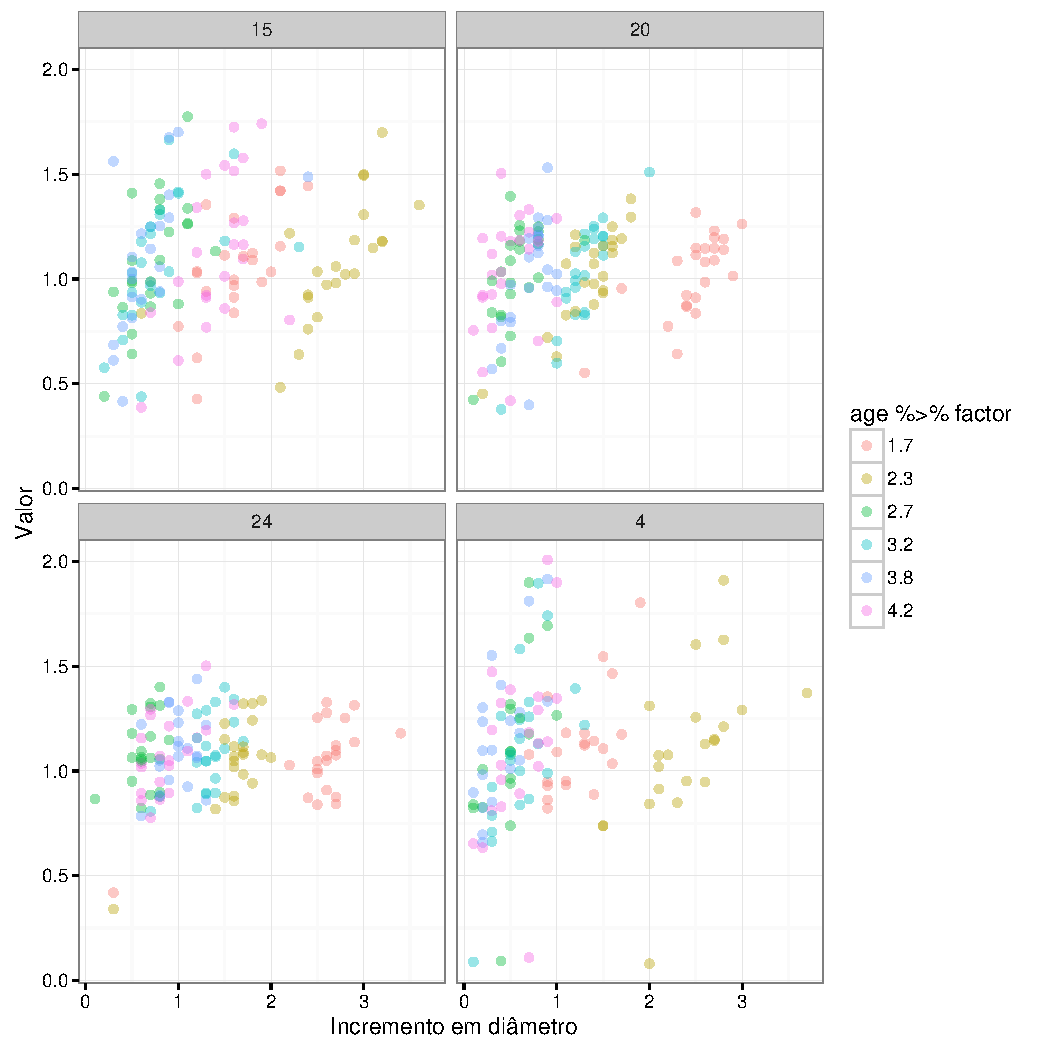
\includegraphics{comp3-paper_files/figure-latex/unnamed-chunk-18-1} \end{center}

\end{CodeChunk}

\begin{CodeChunk}
\begin{CodeInput}
base_index_sml %>% 
  filter(index == "daniels") %>% 
  ggplot(aes(cai, value, color = age %>% factor)) +
    geom_point(alpha = 0.4) +
    facet_wrap(~site) +
    labs(x = ~Incremento~em~diâmetro, y = ~Valor)
\end{CodeInput}


\begin{center}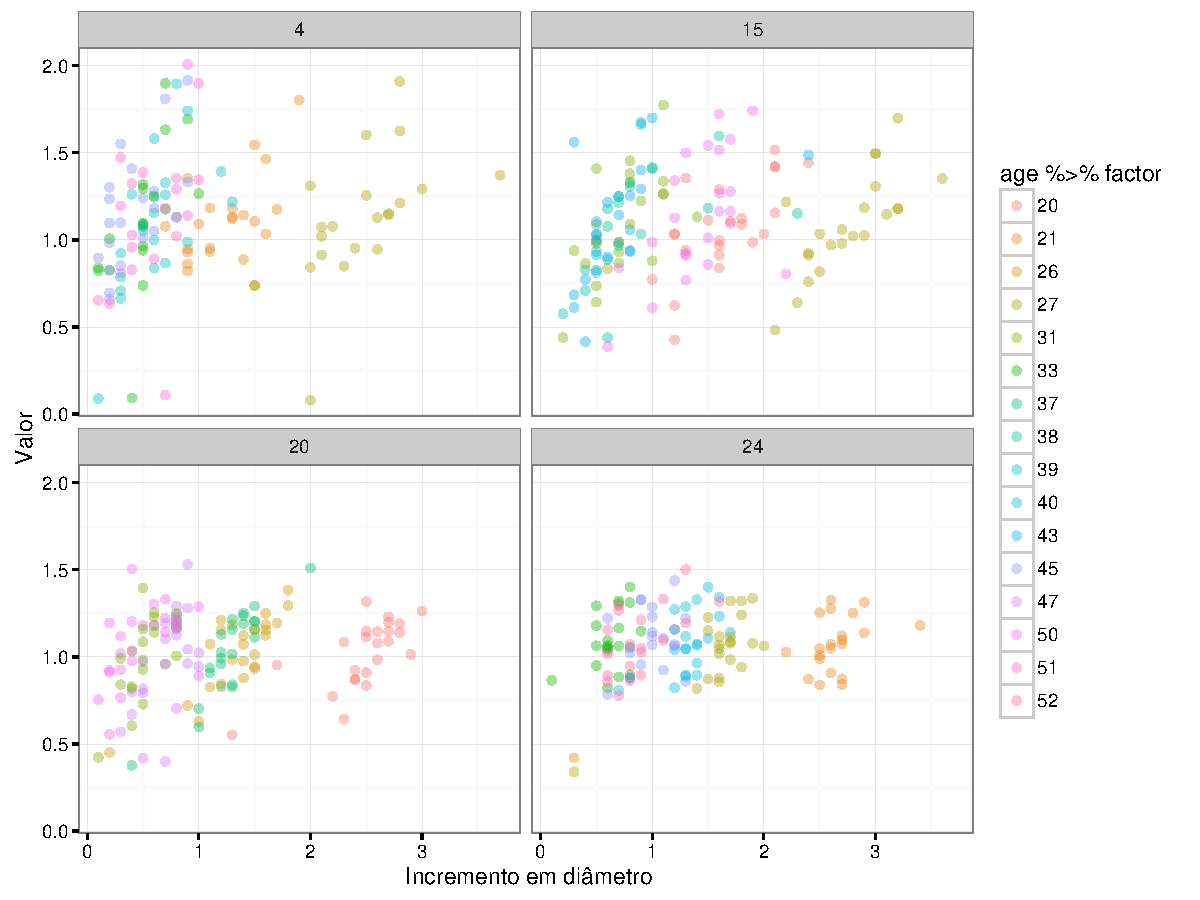
\includegraphics{comp3-paper_files/figure-latex/unnamed-chunk-19-1} \end{center}

\end{CodeChunk}



\end{document}

